\section{Backend}\label{sec:poc:backend}
\begin{figure}[ht]
  \centering
  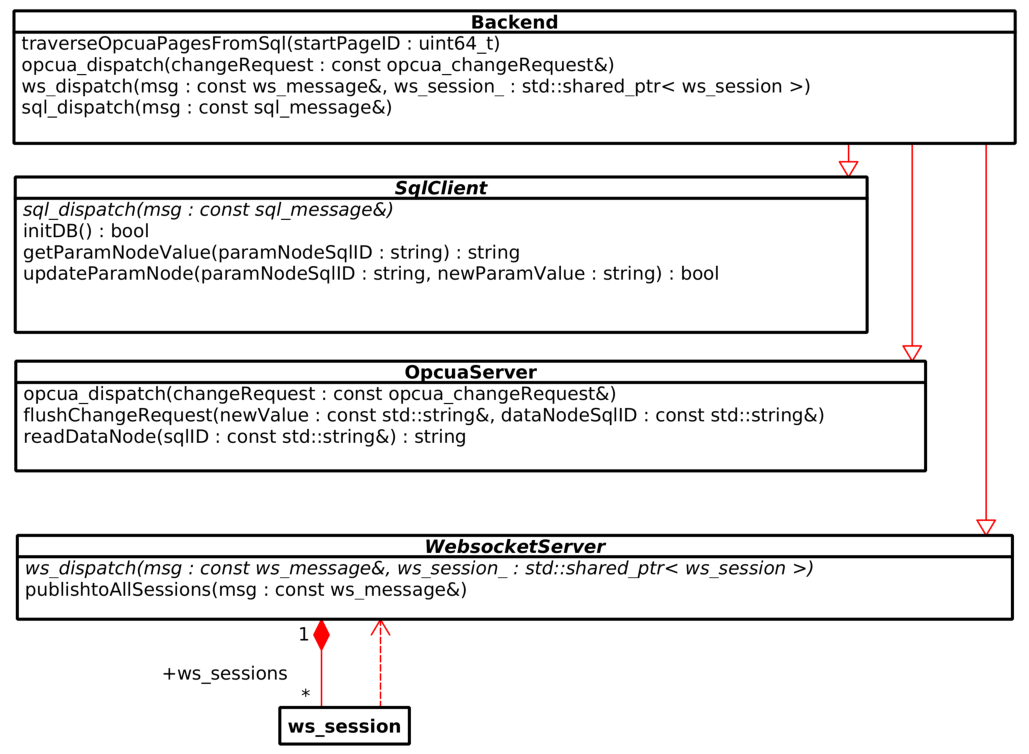
\includegraphics[width=\textwidth]{content/hauptteil/umsetzungPoC/backend/uml/overview.pdf}
  \caption{Klassediagramm Überblick Backend}
  \label{fig:backend:classDiag:overview}
\end{figure}
Das Klassendiagramm in \refFig{fig:backend:classDiag:overview} stellt die Grundstruktur des Backends dar. 
Das Diagramm ist, bis auf die \eigenName{Backend} Klasse, nicht vollständig und auf die wesentlichen Operationen zur Kommunikation reduziert. 
Die \eigenName{Backend} Klasse (abgeleitete Klasse) erbt von den drei Basisklassen \eigenName{SqlClient}, \eigenName{OpcuaServer} und \eigenName{WebsocketServer}.
Jede Basisklasse hat ihre eigene dedizierte Aufgabe die in den einzelnen jeweiligen, gleichnamigen Abschnitten genauer beschrieben ist.
Die abgeleitete Klasse steht dabei als Vermittler dazwischen. Möchte eine der Basisklassen etwas ausführen für das eine der anderen Klassen benötigt wird, 
so kann diese das anstoßen, indem sie eine virtuelle (genauer: \eigenName{pure virtual}) Methode aufruft, die in der Basisklasse selbst nicht implementiert wird, sondern in der abgeleiteten \eigenName{Backend} Klasse.
Dies ermöglicht es nun indirekt durch eine Basisklasse eine Methode einer anderen Basisklasse aufzurufen.
Um zu garantieren, dass dies auch geschieht und nicht durch einen Tippfehler eine falsche Methode aufgerufen wird, 
ist die Methode in der Basisklasse mit \eigenName{ = 0 } definiert, was den Versuch der Dereferenzierung dieser Methode verhindert und mit einem Kompilerfehler kennzeichnet.
Diese Eigenschaft einer Methode ist im Klassendiagramm durch die kursive Schrift der Operation gekennzeichnet.
In der abgeleiteten Klasse (\eigenName{Backend}) wird die dort reimplementierte Methode nun mit dem Schlüsselwort \eigenName{override} am Ende der Deklaration gekennzeichnet.
Dies zwingt den Kompiler zu überprüfen, ob die dort deklarierte Methode wirklich eine Methode der Basisklasse reimplementiert und nicht eine neue Methode ist.
Zusätzlich zu den virtuellen Methoden, die in diesem Fall eine Kommunikation zu anderen Basisklassen, indirekt über die abgeleitete Klasse, ermöglichen, existieren noch eine Anzahl an Methoden, 
über die man mit der Klasse selbst Interagieren kann.
Eine Sonderrolle nehmen dabei die Operationen ein, die im Klassendiagramm von \refFig{fig:backend:classDiag:overview}, noch dargestellt sind.
Sie ermöglichen die Änderung oder Abfrage von Daten der jeweiligen Klassen.
%erwähnung datenaustausch zwischen basisklassen zu abgeleitetrer...(dispatcher.... )
  %endlich anzahl an fkt für daten backend -> basisklassen
  %pro basisklasse ein dispatcher im Backend (virtual) --> Verweis auf Kapitel
%erwähnung message klassen die geparsed wwerden ------- besser in einzelnen abschnitten

Die einzelnen Basisklassen sind zusätzlich separat in den Abbildungen 
\ref{fig:backend:classDiag:WebsocketServer}, \ref{fig:backend:classDiag:SqlClient} sowie \ref{fig:backend:classDiag:OpcuaServer} 
vollständig, mit allen Attributen und Operationen dargestellt.
\subsection{WebsocketServer}

%kurze Erwähnung sinn der klasse
%datenaustausch zwischen WebsocketServer zu abgeleitetrer...(dispatcher.... ) (I/O)
\begin{figure}[ht]
  \centering
  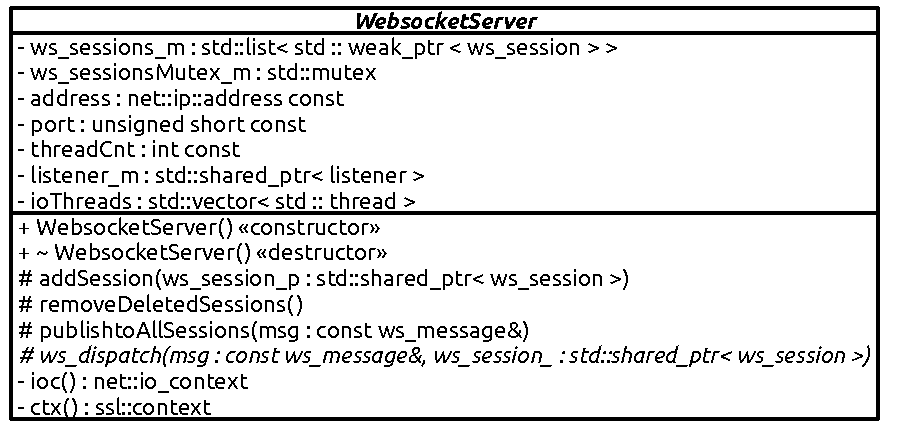
\includegraphics[width=\textwidth]{content/hauptteil/umsetzungPoC/backend/uml/classesOfOverview/WebsocketServer.pdf}
  \caption{Klassediagramm der Klasse \eigenName{WebsocketServer}}
  \label{fig:backend:classDiag:WebsocketServer}
\end{figure}
%beschreibung msg klasse mit diagram
\begin{figure}[ht]
  \centering
  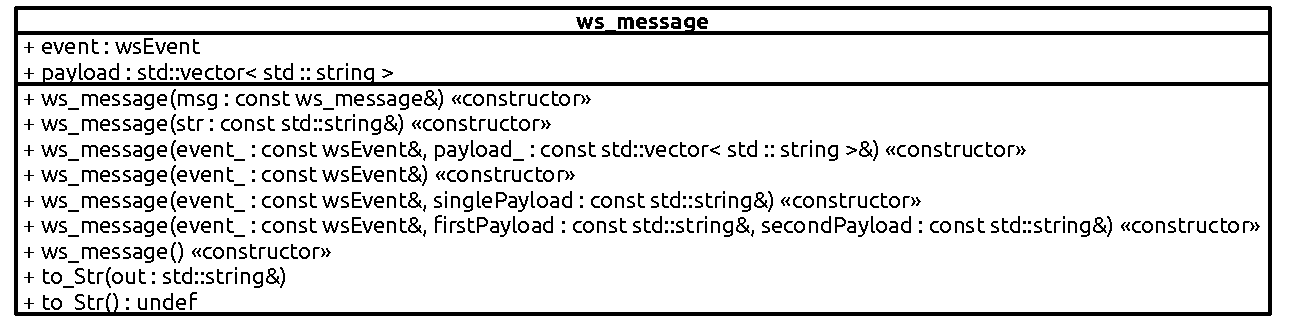
\includegraphics[width=\textwidth]{content/hauptteil/umsetzungPoC/backend/uml/classesOfOverview/ws_message.pdf}
  \caption{Klassediagramm der Klasse \eigenName{ws\_message}}
  \label{fig:backend:classDiag:wsMsg}
\end{figure}
%dispatcher codeausschnitt
%beschreibung dispatcher
\subsection{SqlClient}
%kurze Erwähnung sinn der klasse
%datenaustausch zwischen SqlClient zu abgeleitetrer...(dispatcher.... ) (I/O)
\begin{figure}[ht]
  \centering
  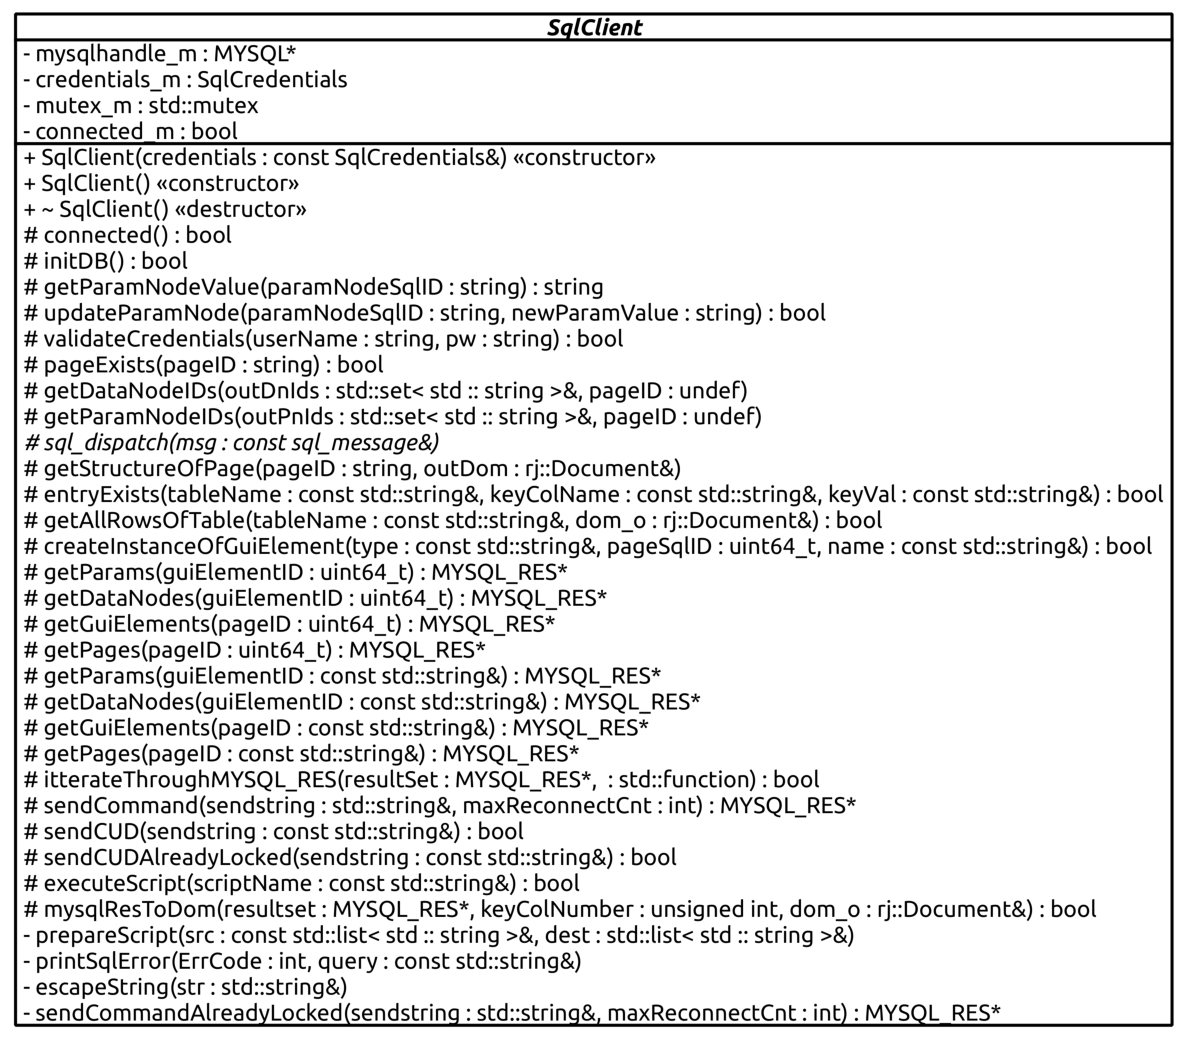
\includegraphics[width=\textwidth]{content/hauptteil/umsetzungPoC/backend/uml/classesOfOverview/SqlClient.pdf}
  \caption{Klassediagramm der Klasse \eigenName{SqlClient}}
  \label{fig:backend:classDiag:SqlClient}
\end{figure}
%beschreibung msg klasse mit diagram
\begin{figure}[ht]
  \centering
  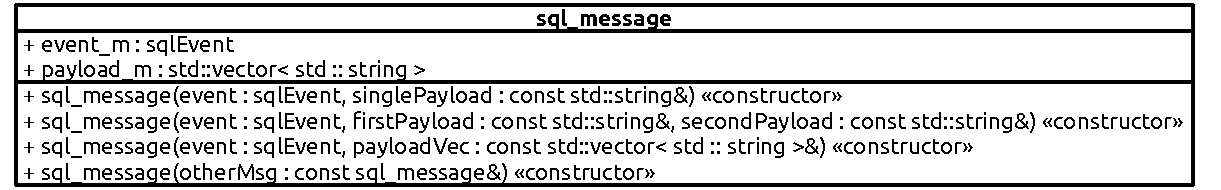
\includegraphics[width=\textwidth]{content/hauptteil/umsetzungPoC/backend/uml/classesOfOverview/sql_message.pdf}
  \caption{Klassediagramm der Klasse \eigenName{sql\_message}}
  \label{fig:backend:classDiag:sqlMsg}
\end{figure}
%dispatcher codeausschnitt
%beschreibung dispatcher
\subsection{OpcuaServer}
%kurze Erwähnung sinn der klasse
%datenaustausch zwischen OpcuaServer zu abgeleitetrer...(dispatcher.... ) (I/O)
\begin{figure}[ht]
  \centering
  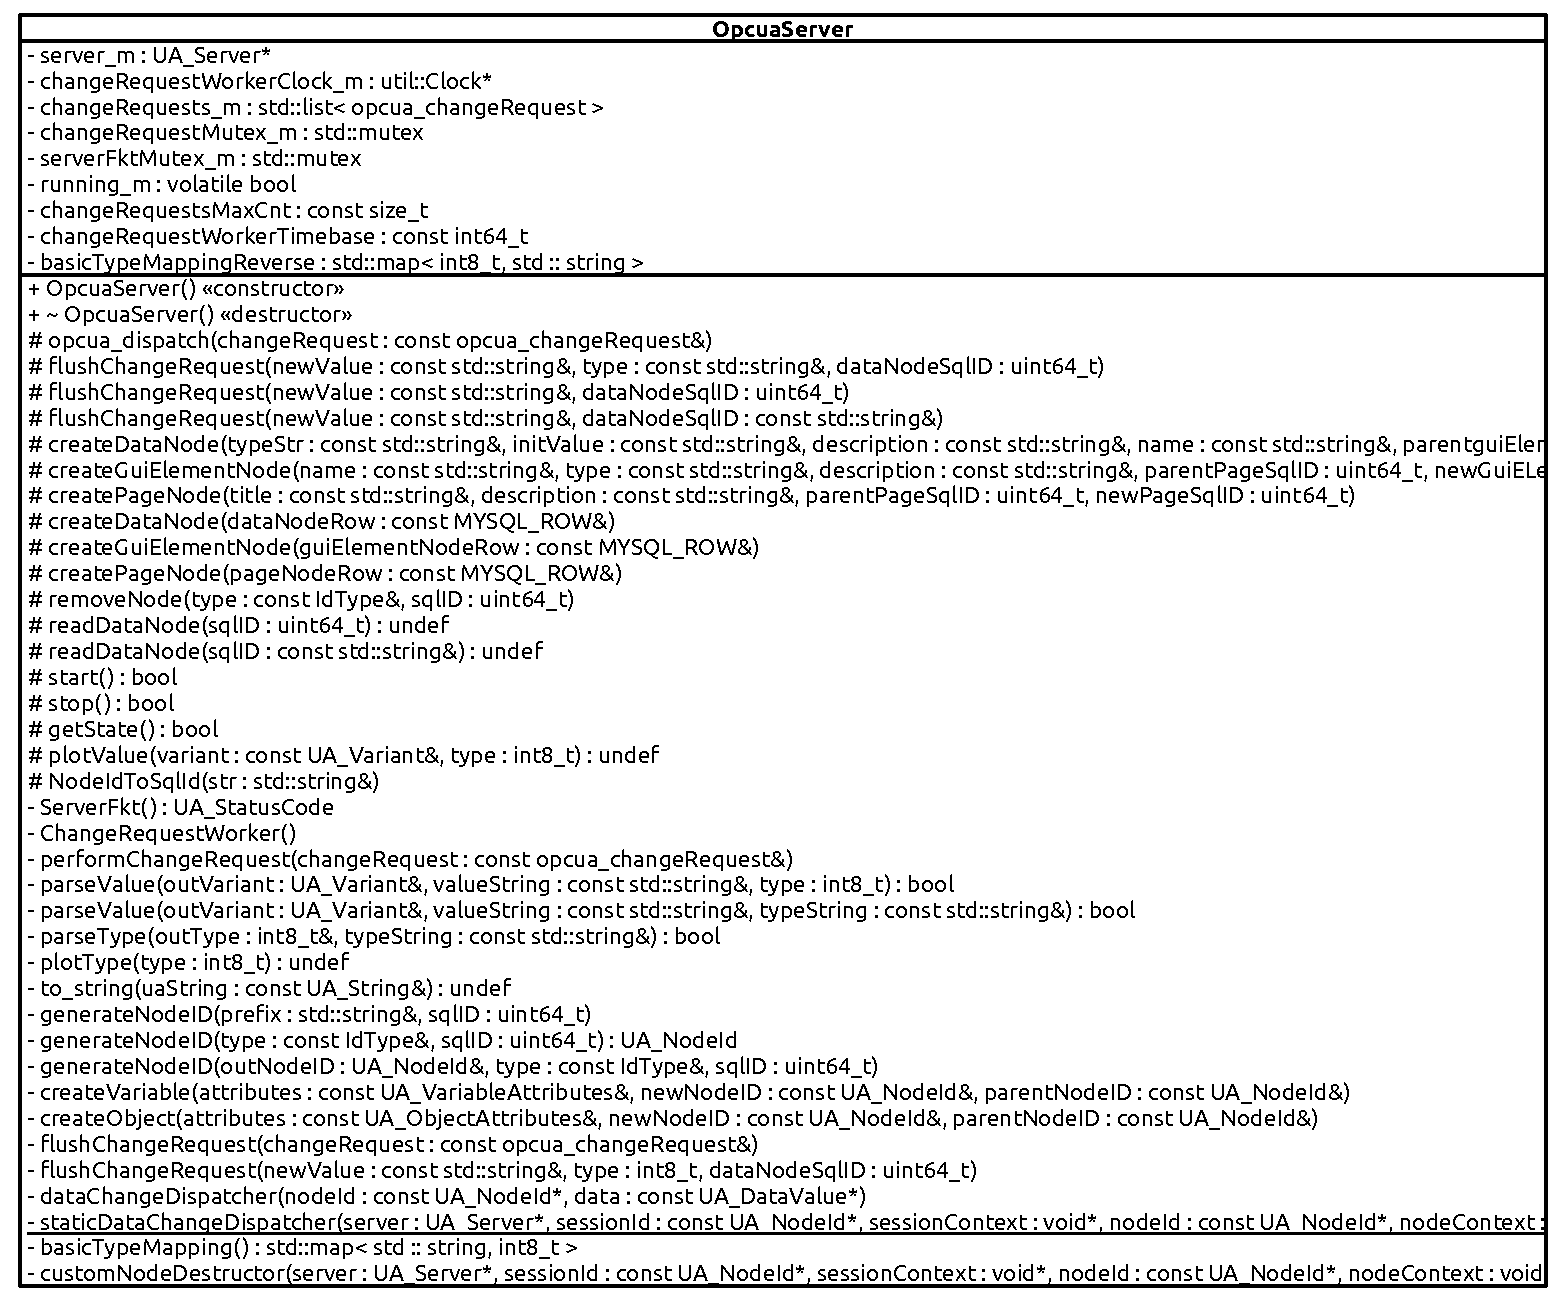
\includegraphics[width=\textwidth]{content/hauptteil/umsetzungPoC/backend/uml/classesOfOverview/OpcuaServer.pdf}
  \caption{Klassediagramm der Klasse \eigenName{OpcuaServer}}
  \label{fig:backend:classDiag:OpcuaServer}
\end{figure}
%beschreibung msg klasse mit diagram
\begin{figure}[ht]
  \centering
  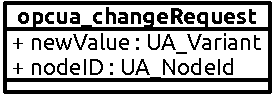
\includegraphics[width=0.2\textwidth]{content/hauptteil/umsetzungPoC/backend/uml/classesOfOverview/opcua_changeRequest.pdf}
  \caption{Klassediagramm der Klasse \eigenName{opcua\_changeRequest}}
  \label{fig:backend:classDiag:opcuaCR}
\end{figure}
%dispatcher codeausschnitt
%beschreibung dispatcher




%%%%BRAINSTORM BABU:
%packete zeigen, beispiele aktionen screenshot chrome wss